\documentclass{article}
\usepackage[letterpaper, margin=1in]{geometry}
\usepackage{graphicx}
\usepackage{amsmath}
\usepackage[backend=bibtex]{biblatex}
\usepackage[hidelinks, linktoc=all]{hyperref}
\usepackage{tikz,tikz-3dplot}
\usepackage[hypcap=false, margin = 3cm]{caption}
\usepackage{booktabs}

\DeclareMathOperator{\Ell}{\mathcal{L}}
\newcommand{\harpoon}{\overset{\rightharpoonup}}

\usetikzlibrary{calc}

\bibliography{references}

\title{Swerve Model}
\author{Justin Turcotte, Austin Schuh}
\date{May 2024}

\begin{document}

\maketitle
\tableofcontents
\newpage
\section{Swerve Model}
\subsection{Single Tire}
This section describes the physics behind a single tire model where all variables are in reference to the wheel. The full robot model is in the next section.
\subsubsection{Definitions}
\begin{center}
    \captionof{table}{Symbol definitions for a Single Tire Model}
    \begin{tabular}{l c c}
        \toprule
        Description                                                           & Symbol     & Units                  \\
        \hline
        Effective Radius of Wheel                                             & $r_e$      & m                      \\
        Longitudinal Velocity                                                 & $v_x$      & m/s                    \\
        Lateral Velocity                                                      & $v_y$      & m/s                    \\
        Angular Velocity of Wheel                                             & $\omega$   & rad/s                  \\
        Angle the velocity vector makes with the longitudinal axis of vehicle & $\theta$   & rad                    \\
        Angle the tire makes with the longitudinal axis of vehicle            & $\delta$   & rad                    \\
        Cornering Tire Stiffness                                              & $C_\alpha$ & N/rad                  \\
        Longitudinal Tire Stiffness                                           & $C_\sigma$ & N                      \\
        Longitudinal Slip Ratio                                               & $\sigma$   & Dimensionless          \\
        Slip Angle                                                            & $\alpha$   & rad                    \\
        Mass                                                                  & m          & kg                     \\
        Gear Ratio(Typically less than 1)                                     & G          & Dimensionless          \\
        External Force in Longitudinal Direction                              & $F_{dx}$   & N                      \\
        External Force in Lateral Direction                                   & $F_{dy}$   & N                      \\
        Current through Motor                                                 & $I$        & A                      \\
        Lateral Force From Tire                                               & $F_a$      & N                      \\
        Longitudinal Force From Tire                                          & $F_o$      & N                      \\
        Motor Torque Constant                                                 & $K_t$      & Nm/A                   \\
        Moment of Inertia of motor to wheel                                   & $J$        & kgm\textsuperscript{2} \\
        \bottomrule
    \end{tabular}
\end{center}
\subsubsection{Tire Forces}
Longitudinal Slip Ratio and Slip angle are defined as follows
\begin{gather}
    \sigma  =  \frac{r_e\omega - v_x}{|v_x|} \\ % add breaking/accelerating and figure out whether we need the abs value
    \alpha = \delta-\theta
\end{gather}
Both of these are empirically proven to be approximately linearly proportional to force around zero. \supercite{tire_basics} Thus
\begin{gather}
    F_o = C_\sigma \sigma \label{f_o}\\
    F_a = C_\alpha \alpha \label{f_a}
\end{gather}
We can also say that
\begin{gather}
    \tan(\theta) = \frac{v_y}{v_x}
\end{gather}
and thus assuming no steering angle, $\delta$, we can say
\begin{gather}
    \alpha = -atan2\left(\frac{v_y}{v_x}\right)
\end{gather}
\subsubsection{Motor Forces}
A DC motor can be modeled by the following two equations
\begin{gather}
    V = IR + \frac{\omega}{K_v}\\
    \tau_{motor} = K_tI \label{motor_torque}
\end{gather}
\subsubsection{Equations of Motion}
We can encapsulate our whole system in terms of $v_x$, $v_y$, and $\omega$(of wheel), thus the total forces in each direction is
\begin{gather}
    \Sigma F_x = F_o + F_{dx}\\
    \Sigma F_y = F_a + F_{dy}\\
    \Sigma \tau = \frac{\tau_{motor} - GF_o r_e}{G}
\end{gather}
The Gear ratios constants are required to shift to and from torque at wheel and motor.
Thus, the equations of motion are
\begin{gather}
    \dot{v}_x = \frac{C_\sigma \frac{r_e \omega - v_x}{v_x} + F_{dx}}{m}\\
    \dot{v}_y = \frac{-C_\alpha atan2\left(\frac{v_y}{v_x}\right) + F_{dy}}{m}\\
    \dot{\omega} = \frac{-GF_or_e + K_tI}{GJ} \label{wheel_omega}
\end{gather}

\subsection{Swerve Model}
\subsubsection{Definitions}

\tdplotsetmaincoords{0}{90}
\begin{center}
    \begin{tikzpicture} [scale=2, tdplot_main_coords, axis/.style={->,blue,thick},
            vector/.style={-stealth,black,very thick},
            vector guide/.style={dashed,black,thick}]

        \coordinate (O) at (0,0);

        \draw[axis] (0,0) -- (0,1) node[anchor=north west]{$\mathbf{v_x}$};
        \draw[axis] (0,0) -- (-1,0) node[anchor=south west]{$\mathbf{v_y}$};

        \draw[thick,tdplot_main_coords] (2,2)-- (2,-2) -- (-2,-2)--(-2,2)--cycle;

        \draw[thick,tdplot_main_coords] (2, 2) node[anchor=south east]{module 3};
        \draw[thick,tdplot_main_coords] (2, -2) node[anchor=south west]{module 2};
        \draw[thick,tdplot_main_coords] (-2, -2) node[anchor=north west]{module 1};
        \draw[thick,tdplot_main_coords] (-2, 2) node[anchor=north east]{module 0};

        \newcommand{\circAr}%
        {  \draw[axis] (0,0, 0) +(0:.25)[->] arc(0:360:.25);
        }

        \begin{scope}[tdplot_main_coords]
            \circAr
        \end{scope}
        \draw[blue, thick](0.35,0,0)node[anchor=west]{$\mathbf{\theta}$};

    \end{tikzpicture}
    \captionof{figure}{Shows the module numbering scheme(like Quadrants) and the axes of the robot}

    \vspace{1cm}

    \tdplotsetmaincoords{0}{90}
    \begin{tikzpicture} [scale=3, tdplot_main_coords, axis/.style={->,blue,thick},
            vector/.style={-stealth,black,thick},
            vector guide/.style={dashed,black,thick},
            ref axis/.style={->,dashed, magenta, thick}]

        %standard tikz coordinate definition using x, y, z coords
        \coordinate (O) at (0,0,0);

        \draw[axis] (0,0,0) -- (0,1,0) node[anchor= west]{$\mathbf{v_x}$};
        \draw[axis] (0,0,0) -- (-1,0,0) node[anchor=west, yshift=-0.15cm]{$\mathbf{v_y}$};
        % \draw[axis] (0,0,0) -- (0,0,1);

        \draw[thick, tdplot_main_coords] (0,0,0) -- (-2, 2, 0) node[midway, anchor = north west]{$\mathbf{\harpoon{d}_{mod}}$};
        \coordinate (perp) at ($ (-2,2,0)!0.15!-90:(0,0,0) $);

        \draw [ref axis] (-2,2,0) -- (perp) node[very near end, anchor = north east]{$\mathbf{\dot{\theta} \times \harpoon{d}_{mod}}$};
        % \draw[thick,tdplot_main_coords] (2,2,0)-- (2,-2,0) -- (-2,-2,0)--(-2,2,0)--cycle;

        \draw[vector guide] (-2,0,0) -- (-2,2,0) node[midway, above]{};
        \draw[vector guide] (0,0,0) -- (-2,0,0) node[midway, above, right, pos=0.65]{};
        \draw[vector guide] (-2,2,0) -- (-2+0.375,2,0);

        \coordinate (Shift) at (-2,2,0);
        \tdplotsetrotatedcoordsorigin{(Shift)}

        \draw[ref axis, tdplot_rotated_coords] (0,0,0) -- (0,0.5,0) node[anchor=north west]{$\mathbf{F_x/v_{mod_x}}$};
        \draw[ref axis, tdplot_rotated_coords] (0,0,0) -- (-0.5,0,0) node[anchor=south]{$\mathbf{F_y/v_{mod_y}}$};
        \draw[ref axis, tdplot_rotated_coords] (0,0,0) -- (0,0,0.5);

        \tdplotsetrotatedcoords{-30}{0}{0}

        \draw[axis, tdplot_rotated_coords] (0,0,0) -- (0,0.5,0) node[anchor= west]{$\mathbf{F_{wy}/v_{patch_y}}$};
        \draw[axis, tdplot_rotated_coords] (0,0,0) -- (-0.5,0,0) node[anchor= west]{$\mathbf{F_{wx}/v_{patch_x}}$};
        \tdplotdrawarc[blue, thick, tdplot_rotated_coords]{(0,0,0)}{0.25}{-60+90}{90}{anchor=north west}{$\mathbf{\psi}$}

        % \newcommand{\circAr}%
        % {  \draw[axis] (0,0, 0) +(0:.25)[->] arc(0:360:.25);
        % }

        % \newcommand{\translatepoint}[1]%
        % {   \coordinate (mytranslation) at (#1);
        % }

        % \translatepoint{0,0,0.5}
        % \begin{scope}[tdplot_main_coords,shift=(mytranslation)]
        %     \circAr;
        % \end{scope}
        % \draw(0,0,0.7)node[anchor=west]{$\psi$};

    \end{tikzpicture}
    \captionof{figure}{Shows the swerve axes one of the module axes, and variables defining the shift in coordinates}

    \captionof{table}{Symbol definitions for the Swerve Model}
    \begin{tabular}{l c c}
        \toprule
        Description                                                   & Symbol                 & Units                  \\
        \hline
        velocity of the module                                        & $\harpoon{v}_{mod}$    & m/s                    \\
        angle of the robot with respect to the field                  & $\theta$               & rad                    \\
        location of the module with respect to a center point         & $\harpoon{d}_{mod}$    & m                      \\
        angular velocity of the robot                                 & $\omega$               & rad/s                  \\
        velocity of the robot                                         & $\harpoon{v}$          & m/s                    \\
        velocity of the contact patch of the wheel                    & $\harpoon{v}_{patch}$  & m/s                    \\
        steer angle of the module                                     & $\theta_{mod_s}$       & rad                    \\
        caster of the wheel                                           & $d_{caster}$           & m                      \\
        angular velocity of steer of a module                         & $\omega_{mod_s}$       & rad/s                  \\
        velocity of the module with respect to the ground             & $\harpoon{v}_{ground}$ & m/s                    \\
        effective radius of the wheel                                 & $r_w$                  & m                      \\
        angular velocity of drive of a module                         & $\omega_{mod_d}$       & rad/s                  \\
        slip ratio of a module                                        & $\sigma_{mod}$         & Unitless               \\
        slip angle of a module                                        & $\alpha_{mod}$         & rad                    \\
        self righting moment of a module                              & $M_{mod_s}$            & m/s                    \\
        force exerted by a module on the robot                        & $\harpoon{F}_{mod}$    & N                      \\
        force of the tire on the module in the Longitudinal direction & $F_{wx}$               & N                      \\
        force of the tire on the module in the lateral direction      & $F_{wy}$               & N                      \\
        mass of the robot                                             & $m$                    & kg                     \\
        moment of inertia of the robot                                & $J_{robot}$            & kgm\textsuperscript{2} \\
        external force on the robot                                   & $\harpoon{F}_d$        & N                      \\
        external torque on the robot                                  & $\tau_d$               & Nm                     \\
        \bottomrule
    \end{tabular}
    \vspace{0.1cm}\\
    Note: Dots on top of symbols represent the time derivative of that symbol. The subscript $mod$ signifies the variable is per module
    \captionof{table}{Symbol definitions for a module of the Swerve Model used in Section 1.2.3 and 1.2.4}
    \begin{tabular}{l c c}
        \toprule
        Description                                                               & Symbol        & Units                  \\
        \hline
        sun angle                                                                 & $\beta$       & rad                    \\
        carrier angle                                                             & $\psi$        & rad                    \\
        planetary angle                                                           & $\gamma$      & rad                    \\
        pitch radius of the sun                                                   & $r_s$         & m                      \\
        pitch radius of the planetary                                             & $r_p$         & m                      \\
        torque on the sun                                                         & $\tau_\beta$  & Nm                     \\
        torque on the carrier                                                     & $\tau_\psi$   & Nm                     \\
        torque on the planetary                                                   & $\tau_\gamma$ & Nm                     \\
        force acting between the sun and planetary                                & $F_1$         & N                      \\
        force acting between the bevel gears                                      & $F_2$         & N                      \\
        force acting on the left axle contact point                               & $F_l$         & N                      \\
        force acting on the right axle contact point                              & $F_r$         & N                      \\
        effective radius of the vertical, smaller bevel gear                      & $r_{b1}$      & m                      \\
        effective radius of the horizontal, larger bevel gear                     & $F_{b2}$      & m                      \\
        offset of the pitch circle of the bevel gear from the center of the wheel & $w_b$         & m                      \\
        distance between the center of the wheel and each axle contact points     & $w_w$         & m                      \\
        torque constant of the motor                                              & $K_t$         & Nm/A                   \\
        current applied to the steer motor                                        & $I_s$         & A                      \\
        current applied to the drive motor                                        & $I_d$         & A                      \\
        moment of inertia of the steer motor                                      & $J_{ms}$      & kgm\textsuperscript{2} \\
        gear ratio from the wheel to steer motor                                  & $G_s$         & Unitless               \\
        gear ratio from the wheel to drive motor                                  & $G_d$         & Unitless               \\
        moment of inertia of the drive motor                                      & $J_{md}$      & Nm                     \\
        gear ratio from the motor to sun                                          & $G_{d1}$      & Unitless               \\
        gear ratio of the sun to planetary gear                                   & $G_{d2}$      & Unitless               \\
        gear ratio of the bevel gears                                             & $G_{d3}$      & Unitless               \\
        angle of the module                                                       & $\theta_s$    & rad                    \\
        angle of the wheel                                                        & $\theta_d$    & rad                    \\
        angle of the wheel motor                                                  & $\theta_{md}$ & rad                    \\
        torque caused by the steer motor on the steer coordinate                  & $\tau_s$      & Nm                     \\
        \bottomrule
    \end{tabular}
\end{center}
\subsubsection{Module Velocities and Forces}
Due to the circular motion, we use a cross product added to linear velocities
\begin{gather}
    \harpoon{v}_{mod} = \left(\omega \times R\left(\theta\right)\harpoon{d}_{mod}\right) + \harpoon{v}\\
    \harpoon{v}_{patch} = \harpoon{v}_{mod} +  \left(\omega + \omega_{mod_s}\right) \times R\left(\theta + \theta_{mod_s}\right)
    \begin{bmatrix}
        d_{caster} \\
        0
    \end{bmatrix}
\end{gather}
where all functions R are rotation matrices expressed as the following
\begin{gather}
    R(\psi) =
    \begin{bmatrix}
        \cos(\psi) & -\sin(\psi) \\
        \sin(\psi) & \cos(\psi)  \\
    \end{bmatrix}
\end{gather}
We then express this in the coordinate system of the wheel which is needed for the tire forces
\begin{gather}
    \harpoon{v}_{ground} = R(-(\theta + \theta_{mod_s}))\harpoon{v}_{patch}
\end{gather}
We then can use those velocities to calculate the slip ratios which are slightly modified
\begin{gather}
    \sigma_{mod} = \frac{r_w\omega_{mod_d} - \harpoon{v}_{ground_x}}{max(0.02, |\harpoon{v}_{ground_x}|)}\\
    \alpha_{mod} = -atan2(\frac{\harpoon{v}_{ground_y}}{\harpoon{v}_{ground_x}})
\end{gather}
The lateral and longitudinal forces are given by equations \eqref{f_o} and \eqref{f_a}.
A tire also has a self aligning torque due to having more forces and the far side of the contact path due to a greater deflection. The equation for this assuming a constant weight distribution is found in \textcite{tire_basics} where $a$ is half the length of the contact patch
\begin{gather}
    M_{mod_s} = -\frac{aF_{wy}}{3}
\end{gather}
\subsubsection{Module Behavior}
{\footnotesize Note: For the following section(until 1.2.4) use symbol table 3 in addition to 2}\\
This section aims to find the static relation, since the inertia is negligible, between the sun gear and the wheel and its relation to the rotation of the whole module
\begin{center}
    % TODO(Justin):A nice latex diagram would be nice at some point intead of an image

    % \tdplotsetmaincoords{60}{100}
    % \begin{center}
    %     \begin{tikzpicture} [scale=2, tdplot_main_coords, axis/.style={blue,thick},
    %             vector/.style={-stealth,black,very thick},
    %             vector guide/.style={dashed,black,thick}]

    %         \coordinate (O) at (0,0);

    %         \draw[axis] (0,0,2) arc (0:360:1);
    %         \draw[axis] (0,2,2) arc (0:360:1);

    %     \end{tikzpicture}
    %     \captionof{figure}{Shows the module numbering scheme(like Quadrants) and the axes of the robot}
    % \end{center}
    \begin{figure}[h]
        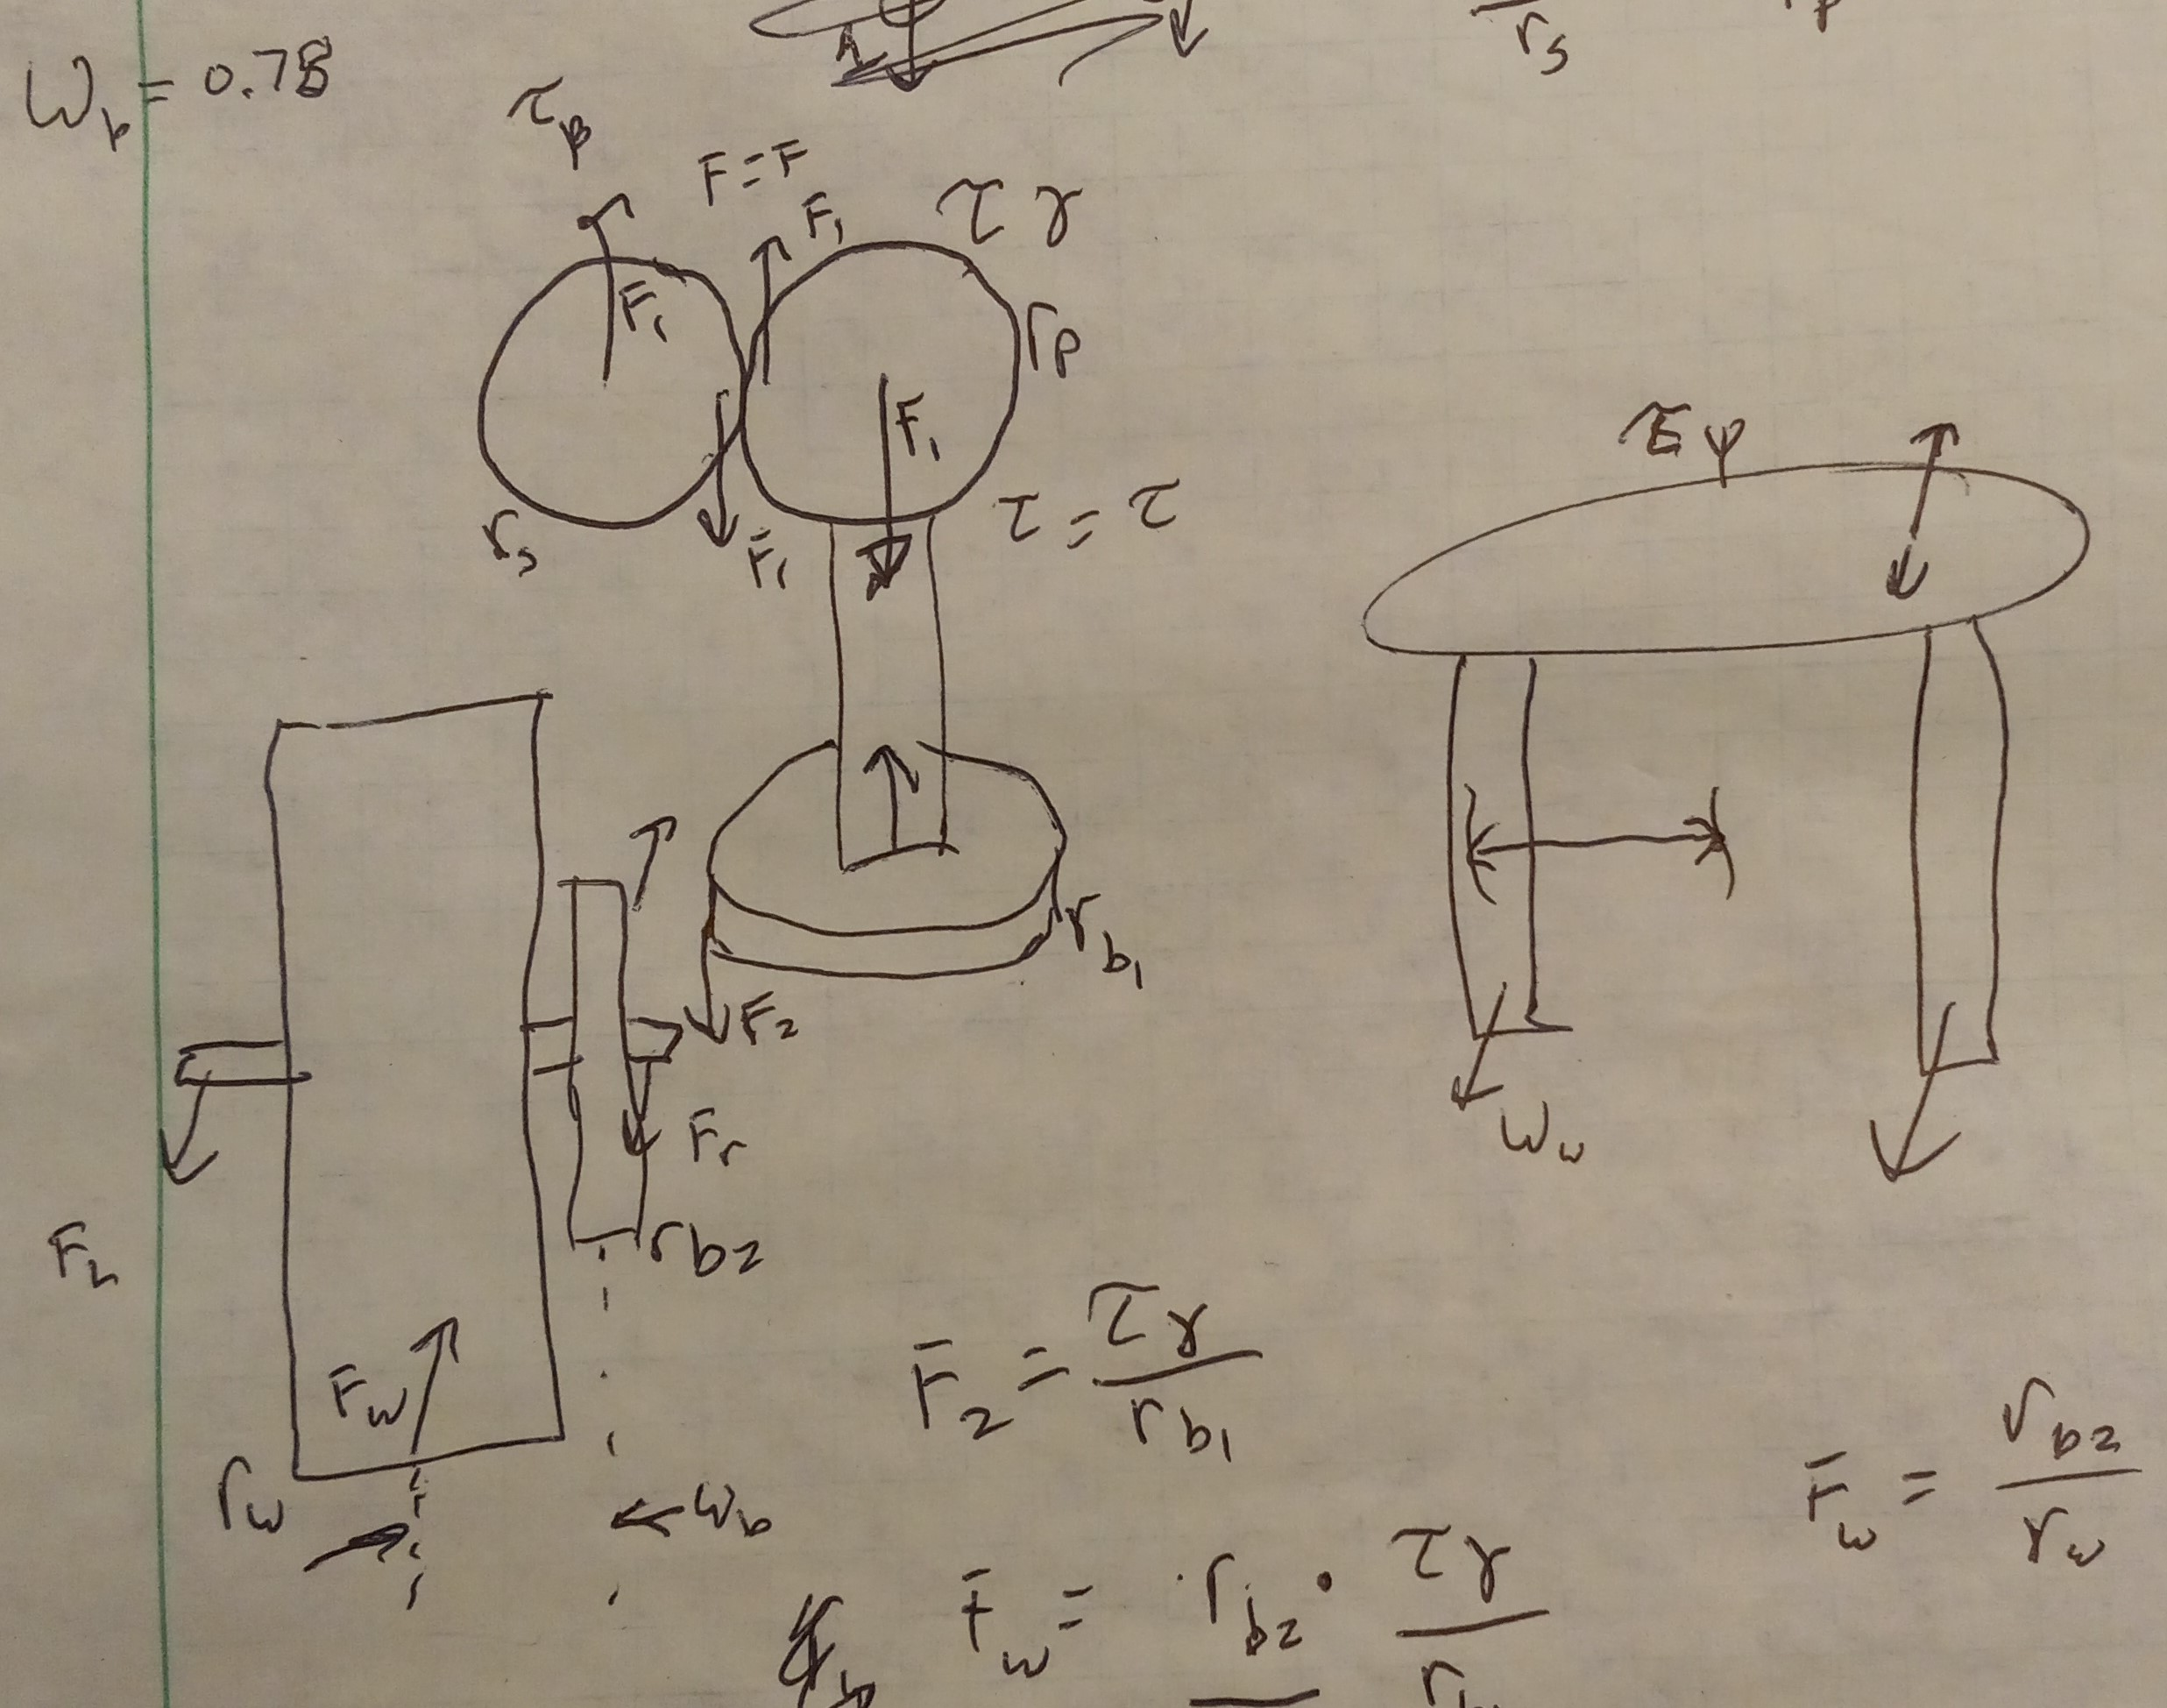
\includegraphics[width=\textwidth]{module_diagram.jpg}
    \end{figure}
    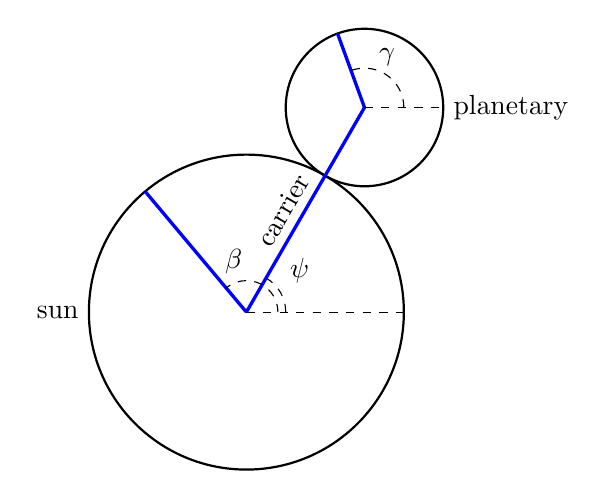
\begin{tikzpicture} [axis/.style={blue, very thick},
            vector/.style={black,thick},
            vector guide/.style={dashed,black}]

        \draw[vector guide] (0.5,0) arc (0:60:0.5) node[midway, anchor = south west]{$\psi$};
        \draw[vector] (2,0) arc (0:360:2) node[midway, anchor = east]{sun};
        \draw[vector] (60:3) ++(1,0) arc (0:360:1) node[anchor = west]{planetary};
        \draw[vector guide] (0,0) --(2,0);
        \draw[axis] (0,0) --(60:3) node[vector, pos=0.45, sloped, above]{carrier};
        \draw[axis] (0,0) -- (130:2);
        \draw[vector guide] (0.4,0) arc (0:130:0.4) node[very near end, anchor = south]{$\beta$};
        \draw[vector guide] (60:3) -- +(1,0);
        \draw[axis] (60:3) -- +(110:1);
        \draw[vector guide] (60:3) ++(0.5, 0) arc (0:110:0.5) node[midway, above]{$\gamma$};
    \end{tikzpicture}
    \captionof{figure}{Each blue line represents a rotational axis where the carrier rotates the planetary gear itself}
\end{center}
From the figure, we can say the following
\begin{gather}
    F_2 = \frac{r_p}{r_{b1}}F_1\\
    F_2 = \frac{\tau_\gamma}{r_{b1}}\\
    F_w = \frac{r_{b2}}{r_w}F_2\label{fw_to_f2}\\
    \tau_\psi +F_lw_w-F_rw_w + \left(r_s+r_p\right)\left(F_2-F_1\right)= 0\label{the_eq}\\
    F_w - F_l -F_r + F_2 = 0
\end{gather}
which we can express as
\begin{gather}
    \left(1+\frac{r_{b1}}{r_w}\right)F_2 - F_l -F_r = 0
\end{gather}
Thus, we can express $F_l$ and $F_r$ in terms of $F_2$
\begin{gather}
    F_l = \frac{1}{2}\left(1+\frac{r_{b1}}{r_w}-\frac{w_b}{w_w}\right)F_2\\
    F_r = \frac{1}{2}\left(1+\frac{r_{b1}}{r_w}+\frac{w_b}{w_w}\right)F_2
\end{gather}
We then plug these values of $F_l$ and $F_r$ into \eqref{the_eq} to express everything in terms of $F_2$ which we can then express in terms of $F_w$ with \eqref{fw_to_f2}
\begin{gather}
    \tau_\psi = \left(w_b + \left(r_s+r_p\right)\left(1-\frac{r_{b1}}{r_p}\right)\right)F_2\\
    = \left(w_b + \left(r_s+r_p\right)\left(1-\frac{r_{b1}}{r_p}\right)\right)\frac{r_w}{r_{b2}}F_w
\end{gather}
\subsubsection{Full Module Kinematics}
We add up all the torques/forces in each dimension to give the following equations. The variables used here are separate per module
\begin{gather}
    M_s + \tau_s + \tau_\psi = J_{total}\ddot{\theta_s}\\
    \tau_md + \tau_d = -F_{wx}r_w\\
    \dot\theta_d = G_{d3}\left(\left(G_{carrier} - 1\right)\dot\theta_s - \dot\theta_{md}G_{motor-to-planet}\right) \label{the_one}
\end{gather}
The $-1$ in equation \eqref{the_one} comes from the additional contirbution of the wrapping around the gear with the change of coordinates.
We can expand this into
\begin{gather}
    M_s + \frac{K_tI_s}{G_s} + \left(-w_b+\left(r_s+r_p\right)\left(1-\frac{r_{b1}}{r_p}\right)\right)\frac{r_w}{r_{b2}}\left(-F_{wx}\right) = \left(J_s + \frac{J_{ms}}{G^2_s}\right)\ddot\theta_s\\
    \frac{J_{md}\ddot\theta_{md}}{G_d}+\frac{K_{t}I_d}{G_d} = F_{wx}r_w \label{md_ddot}\\
    \dot\theta_d = G_{d3}\left(\left(\frac{r_p+r_s}{r_p}-1\right)\dot\theta_s - \dot\theta_{md}G_{d1}G_{d2}\right)
\end{gather}
where each G represents a separate gear ratio.
\subsubsection{Robot Equation of Motion}
We then rotate back the module forces by
\begin{gather}
    \harpoon{F}_{mod} = R(\theta + \theta_{mod_s})\begin{bmatrix}
        F_{wx} \\
        F_{wy}
    \end{bmatrix}
\end{gather}
The linear velocity differential equations are relatively simple as it's just adding all the forces by the module and an arbitrary external force
\begin{gather}
    \dot{\harpoon{v}} = \frac{\Sigma \harpoon{F}_{mod} + \harpoon{F}_{d}}{m}
\end{gather}
However, the angular velocity differential equation is more complicated as the torque added per module varies in sign
\begin{gather}
    \ddot{\theta} = \frac{\Sigma\left(R\left(\theta\right)\harpoon{r} \times \harpoon{F}_{mod}\right) + \tau_{d}}{J_{robot}}
\end{gather}
\subsection{Simplified longitudinal dynamics}

The time constants involved with the longitudinal dynamics are significantly faster than the time constants for accelerating a robot.
This makes the equations pretty stiff and hard to work with.
Ignoring the mass of the wheel, the time constant for a Kraken is around $4ms$.
This also makes it hard on the MPC solver.  Therefore, it is useful to have a simplified version of the physics which solves for the acceleration force directly as a function of drive current.

\eqref{md_ddot} then simplifies to 
\begin{gather}
\frac{K_{t}I_d}{G_d} = -F_{wx}r_w\\
\end{gather}

TODO(austin): Need to document how the position dynamics work for an EKF.

\newpage
\printbibliography
\end{document}
